\documentclass{article}
\usepackage[margin=0.75in]{geometry}
\usepackage{tikz}
\usetikzlibrary{positioning,arrows.meta,calc,fit,backgrounds}
\usepackage{tcolorbox}
\usepackage{xcolor}
\usepackage{skak}

\newcommand{\benchmark}{ChessChain}

\begin{document}

\begin{figure}[t]
    \centering

    % Chess problem - Version 4: Cleaner layout with grouped structure
    \begin{tcolorbox}[
        title=\textbf{Chess: Minimax Search} \hfill {\small\colorbox{orange!20}{Easy} \quad 6 orderings},
        colframe=orange!70!black,
        colback=orange!3,
        boxrule=0.8pt,
        width=\textwidth
    ]
    \small

    \begin{minipage}{0.28\textwidth}
        \centering
        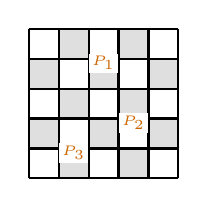
\begin{tikzpicture}[scale=0.38]
            % Draw 5x5 board
            \foreach \x in {0,...,4} {
                \foreach \y in {0,...,4} {
                    \pgfmathparse{mod(\x+\y,2) ? "gray!25" : "white"}
                    \fill[\pgfmathresult] (\x,\y) rectangle (\x+1,\y+1);
                }
            }
            \draw[thick] (0,0) grid (5,5);
            % Knight at (0,4)
            \node at (0.5,4.5) {\small$\symknight$};
            % Pawns with labels
            \node at (2.5,4.5) {\small$\sympawn$};
            \node[font=\tiny, orange!80!black, fill=white, inner sep=1pt] at (2.5,3.85) {$P_1$};
            \node at (3.5,2.5) {\small$\sympawn$};
            \node[font=\tiny, orange!80!black, fill=white, inner sep=1pt] at (3.5,1.85) {$P_2$};
            \node at (1.5,1.5) {\small$\sympawn$};
            \node[font=\tiny, orange!80!black, fill=white, inner sep=1pt] at (1.5,0.85) {$P_3$};
        \end{tikzpicture}

        \vspace{0.15cm}
        {\scriptsize Knight $K$ captures}\\[-0.1cm]
        {\scriptsize all three pawns}
    \end{minipage}%
    \hfill%
    \begin{minipage}{0.70\textwidth}
        \centering
        \textbf{Dependency graph:}
        \vspace{0.15cm}

        \begin{tikzpicture}[
            node distance=0.5cm and 0.7cm,
            every node/.style={font=\scriptsize},
            bfsbox/.style={draw, rounded corners=3pt, fill=orange!10, thick, draw=orange!40, inner sep=4pt},
            treegroup/.style={draw, rounded corners=3pt, fill=orange!22, thick, draw=orange!50, inner sep=5pt},
            outputnode/.style={draw, rounded corners=3pt, fill=orange!45, minimum width=1.1cm, minimum height=0.55cm, thick, draw=orange!70, font=\scriptsize\bfseries},
            arrow/.style={-{Stealth[length=2mm]}, thick, orange!60!black},
            bigarrow/.style={-{Stealth[length=2.5mm]}, line width=1.5pt, orange!50!black}
        ]
            % BFS box (grouped)
            \node[bfsbox] (bfs) {
                \begin{tabular}{@{}c@{}}
                \textbf{BFS distances}\\[2pt]
                $d_{K,P_1}$, $d_{K,P_2}$, $d_{K,P_3}$\\[1pt]
                $d_{P_1,P_2}$, $d_{P_1,P_3}$, $d_{P_2,P_3}$
                \end{tabular}
            };

            % Game tree box (grouped)
            \node[treegroup, below=0.8cm of bfs] (tree) {
                \begin{tabular}{@{}c@{}}
                \textbf{Minimax game tree}\\[3pt]
                \begin{tikzpicture}[
                    scale=0.9,
                    every node/.style={font=\tiny},
                    maxn/.style={draw, circle, fill=orange!15, minimum size=0.4cm, inner sep=0pt, thick, draw=orange!50},
                    minn/.style={draw, rectangle, fill=orange!35, minimum size=0.35cm, inner sep=1pt, thick, draw=orange!60},
                    leafn/.style={draw, circle, fill=orange!50, minimum size=0.25cm, inner sep=0pt, thick, draw=orange!70}
                ]
                    % Root
                    \node[maxn] (r) {};

                    % Level 1 - Alice picks first pawn
                    \node[minn, below left=0.4cm and 0.9cm of r] (a1) {$P_1$};
                    \node[minn, below=0.4cm of r] (a2) {$P_2$};
                    \node[minn, below right=0.4cm and 0.9cm of r] (a3) {$P_3$};

                    % Level 2 - Bob picks second pawn (leaves shown as dots)
                    \node[leafn, below left=0.35cm and 0.15cm of a1] (l1) {};
                    \node[leafn, below right=0.35cm and 0.15cm of a1] (l2) {};
                    \node[leafn, below left=0.35cm and 0.15cm of a2] (l3) {};
                    \node[leafn, below right=0.35cm and 0.15cm of a2] (l4) {};
                    \node[leafn, below left=0.35cm and 0.15cm of a3] (l5) {};
                    \node[leafn, below right=0.35cm and 0.15cm of a3] (l6) {};

                    % Edges
                    \draw[thick, orange!40] (r) -- (a1);
                    \draw[thick, orange!40] (r) -- (a2);
                    \draw[thick, orange!40] (r) -- (a3);
                    \draw[semithick, orange!40] (a1) -- (l1);
                    \draw[semithick, orange!40] (a1) -- (l2);
                    \draw[semithick, orange!40] (a2) -- (l3);
                    \draw[semithick, orange!40] (a2) -- (l4);
                    \draw[semithick, orange!40] (a3) -- (l5);
                    \draw[semithick, orange!40] (a3) -- (l6);

                    % Labels
                    \node[font=\tiny, anchor=west] at ([xshift=0.15cm]r.east) {MAX};
                    \node[font=\tiny, anchor=west] at ([xshift=0.15cm]a3.east) {MIN};
                    \node[font=\tiny, anchor=north] at ([yshift=-0.1cm]l4.south) {$3!=6$ leaves};
                \end{tikzpicture}
                \end{tabular}
            };

            % Output
            \node[outputnode, below=0.8cm of tree] (out) {\textbf{Output}};

            % Big arrows connecting the stages
            \draw[bigarrow] (bfs.south) -- (tree.north);
            \draw[bigarrow] (tree.south) -- (out.north);

        \end{tikzpicture}
    \end{minipage}

    \vspace{0.1cm}
    \hrule
    \vspace{0.1cm}

    \begin{tabular}{@{}p{0.48\textwidth}p{0.48\textwidth}@{}}
    \textit{Step 1:} BFS computes shortest knight moves between all pairs of positions. &
    \textit{Step 2:} Minimax over $3!$ orderings: Alice (MAX) and Bob (MIN) alternate choosing which pawn to capture. \\
    \end{tabular}

    \vspace{0.15cm}
    \hfill \textbf{Answer:} [Redacted]
    \end{tcolorbox}

    \caption{\textbf{Chess dependency graph:} \colorbox{orange!10}{BFS} precomputes all pairwise distances, which feed into the \colorbox{orange!22}{minimax game tree} with $3! = 6$ leaf orderings. Circle = MAX (Alice), square = MIN (Bob), filled circles = leaf evaluations.}
\end{figure}

\end{document}
